\chapter{Dead code identification}
\label{ch:identification}

% - dynamic
% - Still need for static analysis
% - PHP append
% - get_included_files
% - get_executed_functions
% - svn information
% - limitations
% - toolset
% - visualisations

This chapter will explain the different types of dead code and discuss where dead code comes from. In the introduction was already established that dead code leads to a bigger code base which presents an issue for maintenance of the software and therefore should be avoided or removed. After the terminology is clarified the chapter will focus on the granularity of the identified dead code needed to achieve the goal of easier to maintain software. Next the different analysis methods and their implications will be discussed.

\section{Dead code}
\label{sec:dead}

\begin{figure}
	\center
	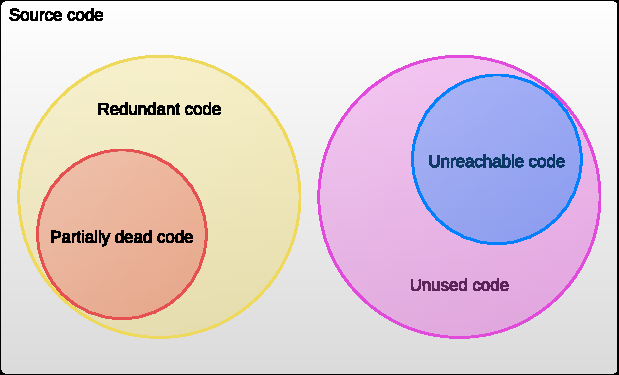
\includegraphics{DeadCodeVenn}
	\caption{\label{fig:deadvenn}Dead code classification, in this thesis dead code is refers to unreachable and unused code}
\end{figure}

The following terminology for dead code is used in literature. 
Knoop\cite{knoop1994} refers to code that is unnecessarily executed when speaking of dead code. Chen\cite{chen1998} calls all code that is not executed on any program path dead code. Janota\cite{janota2007} calls this code unreachable code and code that is unnecessarily executed, redundant code, both subclasses of dead code. Knoop\cite{knoop1994} writes about partial dead code, which is code that is only dead on some program path. 

If looking at dead code we can classify the following sets of dead code: The set of redundant code, code that is executed but does not change the outcome of the program. Partial dead code is a subset of redundant code because it is executed on some paths. Next we have code that is never executed. In this thesis we call this unused code. Some unused code could be executed but never was because the user never used a function to trigger execution of the unused part of the code. Unreachable code would be a subset of unused code. For unreachable code we use the definition of Janota\cite{janota2007}, code that is never executed on any program path. This classification can be seen in \autoref{fig:deadvenn}.

When the term dead code is used in this thesis it refers to unused code, including unreachable code because this is the code we are interested in from a maintenance point of view. From a performance perspective this would not be a problem as long as the source files are not included in the final distribution as is often the case for static languages because the compiler can optimize them out. Redundant code is not included because it can not be determined with dynamic analysis. When we need to be specific the terms partial dead code, redundant code, unused code and unreachable code will be used.

\section{Causes of dead code}

Dead code is not written on purpose, but still almost all applications possess dead code. The following items cause the existence of dead code: 
\begin{description}

\item [Unclear or incomplete specifications] 
Unclear specifications lead to dead code when parts of code are only ran when certain conditions are met. If those conditions are never met in practice because such a case will never arise, those pieces of code are written for nothing due to unclear or incomplete specification. 

\item [Software ageing]
Programming and design mistakes are always made, also in the initial writing of a program. But most arise when changing the software to add new functionality or repair bugs. Changing a program and adding new features will often lead to decay of the structure of an application\cite{parnas1994}. Which in turn will lead to more dead code because programmers are always weary about removing code when they do not have a clear view of the whole program. Dead code because of unused features is a common pattern when software ages. The engineers do not know that certain features are abandoned or simply do not dare remove them\cite{parnas1994,scanniello2011}. When it is known that features are not used any more removing them is not a trivial matter because other parts of the application may have common code with the unused feature. A deep knowledge about the application is required to do so.

\item [Code reuse]
Reuse or reuseability of the software also introduces dead code into an application because not all interfaces and functions will be used\cite{liu1999,tempero2008}.

\item [Modelling objects]
With the introduction of the Object-Oriented programming paradigm it is more likely to model an object and introduce unused methods than with pure procedural code which is only written on demand\cite{srivastava1992}.
\end{description}

\section{Necessary data for dead code identification}

% - granularity
% - collecting information
% - information storage
The first thing to know is what should be measured and to which extent, should statements, methods, classes, components, files or something different be used as smallest unit of dead code, in other words, what will the granularity of the dead code that will be recorded be. The lower the granularity the more information we have available to determine which code is dead. A lower granularity leads to finding more dead code, but also implies more overhead and more data to progress. The overhead should be kept to a minimum and preferable no code should be changed to do the measuring. It is questionable to which extend maintainability can be improved when removing very small pieces of code. Because eliminating dead code needs a lot of effort\cite{andreopoulos2004,jones2006} it is beneficial to start with a large granularity and make it smaller only when there is enough room for improvement left because otherwise too much effort is spend at too little gain. The granularity of dead code identification is a trade-off between overhead and more specific information. We chose the file as smallest unit of dead code to identify. This is part of a top-down approach, first remove dead code at file level and if there is still room for improvement without too much overhead or effort use a smaller unit of dead code, for example a function to get more detailed information.

Because it is impossible to measure dynamically which classes are not used, we measure which classes are used and then take the difference with the set of all classes available in the application. This implies that we can determine which files are dead only after all used files are known. This mean we have to wait until all files that are still in use are expected to be executed. Following conventions used in most languages classes relate to files. Thus if it would be possible to measure included files this would also provide the sought data. The minimum of data that is needed to be able to draw conclusion according a class being alive is coverage\cite{ball1999} data. However to measure how the number of classes in use develops we need more data.  Therefore the first moment in time a class is used should be recorded. It might also be possible that some classes will die within the measurement period. To be able to detect this we also record the last moment in time a class was used. If this date is too far in the past the class can be reckoned dead. Classes that are added to the distribution but still are under development are not likely to be in use and could be mistaken for dead files, it is possible to save the last date a file was changed in the \vcs to solve this problem. To have insight in how many things could be broken when wrongly removing classes from a module, the total number of uses of a class can be saved. This implies a basic form of frequency analysis. This leads to the following list of data to be recorded: number of times used, first time used, last time used, last time edited and changed repository.

\section{Data extraction methods}
% Centralized storage
% Aquire data from multiple sources
% Transform the data
% Aggregate the data
% Modular design
% Adding code to the application
% Registering loaded files or classes
% When to send data to the repository

%dynamic
The data could be acquired by both static and dynamic analysis. But because we look at applications written in dynamic languages and are interested in unused features dynamic analysis is used. 
%The implication of the web application in this context is that all dynamic measurements can be done on a per request base. Because the run-time environment is terminated at the end of each request all used classes (or files) should than be saved.

%aggregate
The data collected should be aggregated directly because storing the raw data would give far too much data to store. Storing raw data could use 1 gibibyte per day for just logging all used files. For example storing 4KiB data $\times$ 4 requests per second $\times$ 3600 seconds per minute $\times$ 24 hours per day = 1.318 GiB per day (Using binary prefixes conforming to \cite{ieee1541}). When measuring applications for multiple months this is simply too expensive. The  4 requests per second is the average that Aurora, the application that will be used for the main use case has during the day. The 4KiB is based on the query size used to update the table in a test set-up for Aurora.

%central
When an application runs on multiple servers or has shared files with other applications the storage should be done on a shared location. All applications send their data to the central repository whereupon the visualizations can be build. 

%recored
There are multiple options to record which files are used by the software. The most generic one is to write a library function which is called from every file upon inclusion of the file. This method can easily be extended to methods, functions and blocks of code. The disadvantage is that adding the function calls can take quite some time if it has to be done by hand. It is possible to the function calls via scripts that automatically add the function calls to the files but it is easy to break things this way. Some scripts may require specific lines to be the first or last in a file which troubles the automatically addition of function calls. When the code base is altered it is very hard to turn everything off and have no overhead any more because all files have to be changed again. An other possibility is to place logging code in the class loading mechanism if the language supports this. This method is preferred over placing function calls in the code because you only have to change the code at one place. The downside is that it is less generic because it can only be used for classes that are dynamically loaded. It is possible to log both classes as well as files that are in use. If the languages uses a garbage collector that can be controlled it is possible to record the elements that were garbage collected. This method has the disadvantage that the objects that are not garbage collected are not added to the set of alive code. If the garbage collector collects all object for the application this could be overcome by calling the garbage collector one last time before exiting the application. The PHP garbage collector can not handle cyclic dependencies\cite{php}, which makes this method not suitable for our use cases.

It is possible that the language at hand offers native support to get a list of all included files, modules or classes. In that case it is possible to use this function and do not worry about all the problems described for the other methods. If a function like this is available this is the preferred method to use. PHP offers this functionality.

%vcs
As described in the section about which data should be available, not only data from the dynamic analysis should be added to the central storage used for the dead code identification but also data from the \vcs should be added. Most \glspl{vcs} can give you the date a file is last edited. This data can be collected and put in the repository as soon as the set of files that will be deployed is known. If possible this should be integrated into the deployment process so that every time that new files are deployed to the production server also new \vcs data is added to the central dead code storage.

%all files
To be able to get from files that are in use by the application to the files that could be dead we need also the set of all files available. This can be achieved by recursively listing the directory contents of the deployed project. In the case of PHP we would only take the \verb|*.php| files into account because we are not interested in non executable files. It is possible to get all available files just before calculating which files are dead but if they are put in the database upfront it is possible to always select which files are used and which are not. This also adds the possibility to create an index of all the files so that the usage information can be processed quickly instead of having to add new files and re-index when more files are used. The performance will stay the same over time when all files are added to the index upfront. Performance will only decrease when more files are added to the application and the index.

%send
Besides collecting all used files, this data also has to be send to the database at some time. Because we are working with web applications the process length is limited to one request form the web browser.   
This leads to the simple decision to send the file names of the used files to the database at the end of each request. This way a minimum number of requests to the database has to be made. 

%Not all languages for the web use the scheme with separated processes per thread. Web applications written in Java and are loaded into memory and handle all requests. For these applications it is possible to select a different moment in to to update the database containing dead code information. For performance reasons it could be beneficial to send the data less often, but sending the data at every request makes sure that if the application crashes there will not be much information lost.

%Foreward reference to visualization
Only recording which code is dead is not enough, the dead code also has to be visualized in a way that is easy for the user to understand and easy to extend when more features or data sets are needed. Therefore the main visualization is build in PHP and javascript as web application. To prevent developers using (possible) dead files by mistake those files should preferably be marked in the \ide{}. More on the visualization can be found in the chapter on visualization (chapter \ref{ch:visualization})

\section{Approach used in this thesis}
For this thesis we use the term dead code for code that is not executed\cite{chen1998}, this includes unused and unreachable\cite{janota2007} code. Redundant code\cite{janota2007} and partial dead code\cite{knoop1994} is not included. Dead code is caused by software ageing\cite{parnas1994,scanniello2011}, code reuse\cite{liu1999,tempero2008}, object modelling\cite{srivastava1992} and unclear specifications. For performance and cost of maintenance\cite{andreopoulos2004,jones2006} the dead files will be identified. If a more fine grained approach is needed this can be done on the files not yet removed. This is left as future work. The data needed to draw conclusions consists of the path of the file, how often it was used and when it was used for the first and last time. \vcs data about when the file was last modified is also added to prevent removing new features that are already in the production system but not activated. The dead files can be detected by recording which files are in use and subtract those from all files. To detect the files in use multiple methods consist. The best one is to rely on a language feature that gives all included files, if this is not possible the class loader or garbage collector could be modified and as last resort calls to a logging function can be added to all files. Because of the amount of data that will be collected everything has to be aggregated right from the start. If the applications are deployed to multiple production servers a centralized storage for the usage data of the files is necessary.

The tools to do this should be very modular so multiple ways of input are possible and the visualizations can easily be reused. The toolbox should allow easy porting to other languages and still be able to use the parts that acquire for example \vcs data.